\section{Sesión 3}
% SESSION III: DEFENSE AGAINST ADVERSARIAL ATTACKS IN FL

Para esta sesión, se ha utilizado de nuevo la configuración de entrenamiento DFL non-IID con la presencia de un nodo malicioso realizando \textit{model poisoning}, tal y como se definió en la sesión anterior. Sobre este escenario, se han evaluado dos mecanismos de agregación robusta con el objetivo de mitigar el impacto de actualizaciones adversarias:

\begin{itemize}
    \item Agregación mediante \textit{Trimmed Mean}.
    \item Agregación mediante \textit{Krum}.
\end{itemize}

\subsection{Trimmed Mean}

El algoritmo \textit{Trimmed Mean} consiste en eliminar un porcentaje de los valores más extremos (potencialmente maliciosos) antes de realizar la agregación de los modelos, reduciendo así la influencia de outliers.

\vspace{1mm}

Los resultados se muestran en la Figura \ref{fig:trimmed_mean}:

\vspace{1mm}
\noindent
\begin{minipage}{\textwidth}
    \centering
    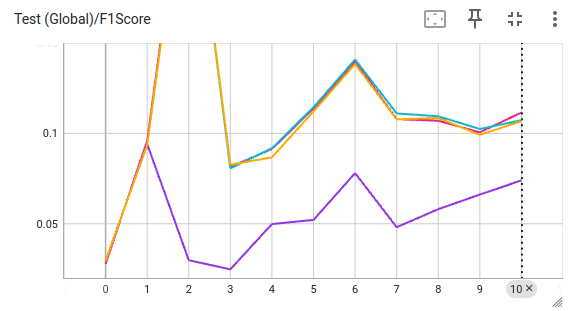
\includegraphics[width=0.5\textwidth]{images/trimmed_mean.png}
    \captionof{figure}{Resultados del entrenamiento con agregación \textit{Trimmed Mean}.}
    \label{fig:trimmed_mean}
\end{minipage}
\vspace{1mm}

Se observa que este método consigue mitigar parcialmente el efecto del nodo malicioso:

\begin{itemize}
    \item El modelo converge de manera relativamente estable, evitando las oscilaciones bruscas observadas en \textit{model poisoning} sin defensa.
    \item El F1-score final se sitúa en torno a 0.11--0.12, lo que supone una mejora significativa frente al caso atacado sin mecanismos de defensa.
    \item Sin embargo, el rendimiento sigue siendo inferior al escenario sin ataques, indicando que el filtrado de valores extremos no elimina completamente el impacto adversario.
\end{itemize}

% Las matrices de confusión muestran una mejora global en la clasificación respecto al escenario atacado, aunque persisten errores distribuidos entre varias clases.

Punto clave: TrimmedMean usa beta=0 por defecto en trimmedmean.py:15, y no vi que backend lo configure. Con beta=0, no recorta extremos y termina en media simple por componente en trimmedmean.py:37.
Además, ese TrimmedMean no pondera por tamaño de dataset (solo promedia tensores), mientras FedAvg sí pondera por muestras en fedavg.py:23 y fedavg.py:33.
Krum aquí selecciona un único modelo (el de menor suma de distancias) en krum.py:44 y krum.py:49; no pondera por muestras y puede tirar mucha información útil en non-IID.


\subsection{Krum}

El algoritmo \textit{Krum} selecciona la actualización más representativa entre los nodos, basándose en la distancia entre modelos, con el objetivo de descartar aquellos que se alejan significativamente (potencialmente maliciosos).

\vspace{1mm}

Los resultados se presentan en la Figura \ref{fig:krum}:

\vspace{1mm}
\noindent
\begin{minipage}{\textwidth}
    \centering
    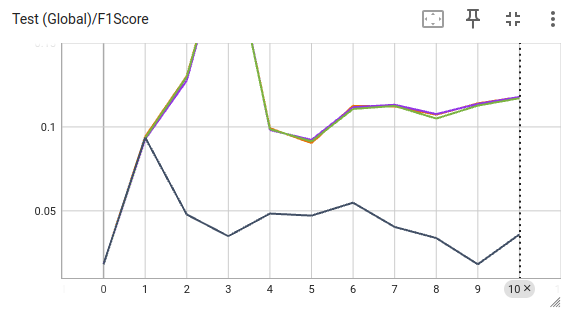
\includegraphics[width=0.5\textwidth]{images/krum.png}
    \captionof{figure}{Resultados del entrenamiento con agregación \textit{Krum}.}
    \label{fig:krum}
\end{minipage}
\vspace{1mm}

En este caso, el comportamiento es diferente:

\begin{itemize}
    \item El entrenamiento es más estable que en el caso sin defensa, pero presenta mayor variabilidad que \textit{Trimmed Mean}.
    \item El F1-score final se sitúa aproximadamente entre 0.07 y 0.11 dependiendo del nodo, mostrando un rendimiento ligeramente inferior en promedio.
    \item Esto sugiere que, aunque Krum es capaz de descartar actualizaciones maliciosas, puede verse afectado por la heterogeneidad non-IID, seleccionando modelos que no representan adecuadamente la distribución global.
\end{itemize}

% Las matrices de confusión reflejan una mayor dispersión en los errores, indicando que el modelo puede estar sesgado hacia ciertas clases dependiendo del nodo seleccionado en cada ronda.

\subsection{Comparación y análisis}

A partir de los resultados obtenidos, se pueden extraer las siguientes conclusiones:

\begin{itemize}
    \item \textit{Trimmed Mean} demuestra una mayor robustez frente a ataques de \textit{model poisoning}, ya que consigue estabilizar la convergencia y alcanzar un F1-score superior en promedio.
    % \textbf{Mayor resiliencia:} 
    \item En escenarios con datos heterogéneos, \textit{Krum} puede verse penalizado, ya que la variabilidad entre nodos puede confundirse con comportamiento malicioso, afectando negativamente a la selección de modelos.
    % \textbf{Impacto de non-IID:} 
    %\item Ninguno de los métodos elimina completamente el efecto del atacante. En \textit{Krum}, se observa un mayor sesgo hacia ciertas clases, lo que sugiere un posible sobreajuste local dependiendo del nodo seleccionado. En \textit{Trimmed Mean}, los errores son más uniformes, indicando un comportamiento más equilibrado.
    % \textbf{Rendimiento por clases:} 
    \item  Ambos métodos mejoran claramente el rendimiento respecto al escenario atacado sin defensa (F1-score $\leq 0.09$), pero no alcanzan los niveles del escenario sin ataques. Esto confirma que, aunque las técnicas robustas ayudan, no eliminan completamente el efecto adversarial.
    % \textbf{Comparación global:}
\end{itemize}

%En conjunto, \textit{Trimmed Mean} resulta más adecuado en este escenario concreto, al ofrecer un mejor equilibrio entre robustez y estabilidad en presencia de nodos maliciosos y datos non-IID.